% License
% This template is derived from the LaTeX template by Florian Walch and contributors available via https://github.com/fwalch/tum-thesis-latex
% This template is licensed under a Creative Commons Attribution-ShareAlike 4.0 International License (see https://creativecommons.org/licenses/by-sa/4.0/), meaning that:
%  * You can share (copy, redistribute) and adapt (remix, transform, build upon) this template for any purpose, even commercially.
%  * If you share the template or a modified (derived) version of it, you must attribute the template to the original authors (Florian Walch and contributors) by providing a [link to the original template][https://github.com/fwalch/tum-thesis-latex] and indicate if changes were made.
%  * Any derived template has to use the samelicense or a compatible license.

\RequirePackage[l2tabu,orthodox]{nag}

\documentclass[headsepline,footsepline,footinclude=false,fontsize=11pt,paper=a4,listof=totoc,bibliography=totoc,BCOR=12mm,DIV=12]{scrbook}

\usepackage[utf8]{inputenc}
\usepackage[T1]{fontenc}
\usepackage[ngerman,english]{babel} % english is the same as american or USenglish
\usepackage{longtable}
\usepackage[]{classicthesis}
\usepackage{booktabs}
\usepackage{graphicx}
\usepackage{subfig} % for having figures side by side
\usepackage[autostyle]{csquotes}
\usepackage{comment}
\usepackage{float}
\usepackage[%
  backend=biber,
  url=true,
  style=numeric, % alphabetic, numeric
  sorting=none, % default == nty, https://tex.stackexchange.com/questions/51434/biblatex-citation-order
  maxnames=4,
  minnames=3,
  maxbibnames=99,
  giveninits,
  uniquename=init]{biblatex} % TODO: adapt citation style

\bibliography{bibliography}

% Settings for search order of pictures
\graphicspath{
    {logos/}
    {figures/}
}

% ************** Math commands *********************
\newcommand{\N}{\ensuremath{\mathbb{N}}}
\newcommand{\R}{\ensuremath{\mathbb{R}}}
\newcommand{\Q}{\ensuremath{\mathbb{Q}}}
\newcommand{\C}{\ensuremath{\mathbb{C}}}
\newcommand{\norm}[1]{|\negthinspace|{#1}|\negthinspace|}
\newcommand{\scp}[2]{\langle #1,\,#2\rangle}
\newcommand{\Mat}[1][n\times n]{\ensuremath{\R^{#1}}}
\newcommand{\definedas}{\mathrel{:=}}
\newcommand{\asdefined}{\mathrel{=:}}
\newcommand{\vect}[2]{\begin{pmatrix}	#1\\#2 \end{pmatrix}}
\newcommand{\vectt}[3]{\begin{pmatrix}	#1\\#2\\#3 \end{pmatrix}}
\newcommand{\vecttt}[4]{\begin{pmatrix}	#1\\#2\\#3\\#4 \end{pmatrix}}
\newcommand{\abs}[1]{\lvert #1 \rvert}
\renewcommand{\ker}{\ensuremath{\text{Kern}\,}}
\newcommand{\bild}{\text{Bild}\,}
\newcommand{\grad}{\text{grad}\,}
\newcommand{\rang}{\text{rang}\,}

% ************** New functions **************




\usepackage{blindtext}
\usepackage{comment}
\usepackage{url}
\usepackage{makecell}
\usepackage{longtable}
\usepackage{amsmath}
\usepackage{subfig}

\begin{document}

% TODO: decide on used language
% \selectlanguage{ngerman}
\selectlanguage{english}

% Set page numbering to avoid "destination wit	h the same identifier has been already used" warning for cover page.
% (see https://en.wikibooks.org/wiki/LaTeX/Hyperlinks#Problems_with_Links_and_Pages).
\pagenumbering{alph}
\frontmatter{}

\definecolor{azulUC3M}{RGB}{0,0,102}
\microtypesetup{expansion=false}

\begin{titlepage}
	\begin{sffamily}
	\color{azulUC3M}
	\begin{center}
		\begin{figure}[H] % UC3M Logo
			\makebox[\textwidth][c]{
\includegraphics[width=16cm]{logos/logo_UC3M.png}}
		\end{figure}
		\vspace{2.5cm}
		\begin{Large}
			Master in Statistics for Data Science\\			
			 2024-2025\\ % Academic year
			\vspace{2cm}		
			\textsl{Master Thesis}
			\bigskip
			
		\end{Large}
		 	{\Huge ``Mixed Integer Stochastic Optimization of relative Position of two Wind Turbines using using Neural Network based Constraint Learning''}\\
		 	\vspace*{0.5cm}
	 		\rule{10.5cm}{0.1mm}\\
			\vspace*{0.9cm}
			{\LARGE Simon Schmetz}\\ 
			\vspace*{1cm}
		\begin{Large}
			Carlos Ruiz Mora\\
			\vspace*{0.5cm}
			Madrid the 29. of January\\
		\end{Large}
	\end{center}
	\vfill
	\color{black}
	\fbox{
	\begin{minipage}{\linewidth}
    	\textbf{AVOID PLAGIARISM}\\
    	\footnotesize{The University uses the \textbf{Turnitin Feedback Studio} for the delivery of student work. This program compares the originality of the work delivered by each student with millions of electronic resources and detects those parts of the text that are copied and pasted. Plagiarizing in a TFM is considered a  \textbf{\underline{Serious Misconduct}}, and may result in permanent expulsion from the University.}\end{minipage}}

	% IF OUR WORK IS TO BE PUBLISHED UNDER A CREATIVE COMMONS LICENSE, INCLUDE THESE LINES. IS THE RECOMMENDED OPTION.
	\noindent
\includegraphics[width=4.2cm]{logos/creativecommons.png}\\ % Creative Commons Logo
    \footnotesize{This work is licensed under Creative Commons \textbf{Attribution – Non Commercial – Non Derivatives}}
	
	\end{sffamily}
\end{titlepage}

%\newpage % blank page
%\thispagestyle{empty}
%\mbox{}
%
%\newpage % blank page
%\thispagestyle{empty}
%\mbox{}

\makeatletter
\ifthenelse{\pdf@strcmp{\languagename}{english}=0}
{\addcontentsline{toc}{chapter}{Acknowledgments}}
{\addcontentsline{toc}{chapter}{Danksagungen}}
\makeatother
\thispagestyle{empty}

\vspace*{20mm}

\begin{center}
\makeatletter
\ifthenelse{\pdf@strcmp{\languagename}{english}=0}
{\usekomafont{section} Acknowledgments}
{\usekomafont{section} Danksagungen}
\makeatother
\end{center}

\vspace{10mm}

%TODO: Acknowledgments
TODO Acknowledgments

\cleardoublepage{}
 % TODO: if you don't have anyone to thank for or don't wish to publish it, comment this line out.

\chapter{\abstractname}

The contents of this thesis are the conceptualization and implementation of a database for computational fluid dynamics data and a fusion algorithm for the fusion of wind tunnel and computational fluid dynamics aerodynamic data. The data consist of polars for coefficients of forces and torques over the angle of attack and the angle of sideslip and is based on Eurofighter Typhoon aerodynamic testing. A relational database structure is implemented and performance tested to store the simulation data, after which two Gaussian process-based approaches, weighted by the uncertainty associated to the aerodynamic data, are pursued for fusion. One approach is based on merging probability density functions resulting from separate Gaussian process models for both sources, which is discarded in favor of the approach to jointly train the Gaussian process regression on both data sources. The ability to fuse two data sources weighted by their associated uncertainty via Gaussian processes is shown and an initial application to the aerodynamic polar data is performed.


\makeatletter
\ifthenelse{\pdf@strcmp{\languagename}{english}=0}
{\renewcommand{\abstractname}{Kurzfassung}}
{\renewcommand{\abstractname}{Abstract}}
\makeatother
\microtypesetup{protrusion=false}
\tableofcontents{}
\microtypesetup{protrusion=true}

\mainmatter{}

%Chapter inputs -------------------------------------------------------------------------------------
% !TeX root = ../main.tex
% Add the above to each chapter to make compiling the PDF easier in some editors.

\chapter{Introduction}\label{chapter:introduction}

Abstract: 

In the following thesis, an attempt is made to combine Linear Optimization with Constraint Learning to optimize the positioning of a fixed number wind turbines in a predifined areal for optimized performance output for randomly distributed wind. To do so, first a Neural Network is trained on simulated data to learn the effects of relative turbine positioning on power output. The model is then introduced as constraint to a linear optimization problem to optimize turbine positioning. The optimal solution is than calculated for a current state of the art optimized windfarm configuration and the results compared. 



Introduction: 

With the clean energy transition currently taking place in europe with ambitious targets for 2030 and beyond (https://energy.ec.europa.eu/topics/renewable-energy/renewable-energy-directive-targets-and-rules/renewable-energy-targets_en#:~:text=The%20revised%20Renewable%20Energy%20Directive,to%20a%20minimum%20of%2042.5%25.&text=The%20energy%20sector%20is%20responsible,the%20EU%27s%20greenhouse%20gas%20emissions.)
, wind energy is playing a central role in that transition, with wind energy expected rise to 50 \% in the EU energy mix (https://www.consilium.europa.eu/media/1kyk0wjm/2024_685_art_windpower_web.pdf). With wind energy thus expected to become the main contributer to the EU's energy production and large potentials identified for both onshore and offshore parks (https://www.eea.europa.eu/en/analysis/publications/europes-onshore-and-offshore-wind-energy-potential), attempts to optimize all parameters of windparks with even minor power efficeny improvement can be expected to yield significant returns in absolute power due to the scale of future wind energy production. 

As a contribution to increasing power efficeny on future wind farms, this thesis is dedicated to a new approach for optimizing the placement of a fixed number of wind turbines in a predefined area (typically a square).

FIG: Wind Park birdseye

To solve this optimization problem, a extension to the pyomo python library is used, that allows the introduction of Neural Networks to the optimization problem as constraints (Constraint Learning, https://www.sciencedirect.com/topics/computer-science/constraint-learning#:~:text=Constraint%20learning%20refers%20to%20the,performance%20in%20computer%20science%20applications.)
. This extension allows for introducing a Neural Neural Network to model the effects of wind turbine placement relative to each other on power production for the respective windturbines. Introducing this model to the optimization problem defined in pyomo then allows for the optimization of overall power productions across all wind turbines in the wind park. To create a model optimally fit to the needs of the optimization problem, the model is trained on data specifically generated with the FLORIS wind farm simulation tool (https://www.nrel.gov/wind/floris.html) for optimal coverage of the parameter space of the optimization. (HOW IS THE MODEL VALIDATED ?)

To simplify the problem, the surface below the turbines is assumed to be perfectly flat and equal wind speed is assumed along the entire hight of the turbines. 

Data Generation and Neural Network: 

(...)

Optimization Problem: 

(...)


This thesis is structued according to the two main steps required to solve the optimization problem as presented above.









% !TeX root = ../main.tex
% Add the above to each chapter to make compiling the PDF easier in some editors.

\chapter{State of the Art}\label{chapter:state_of_the_art}

Since the arrival of large-scale wind turbine farm operations as part of energy infrastructure, optimizing the positioning of the individual wind turbines relative to each other to mitigate wake effects and reduce the total power output is the subject of scientific investigation. As this Thesis is an attempt to apply a novel constraint learning method introduced by Alcantara and Ruiz in \cite{ALCANTARA2023120895} to the optimization of wind farm layouts, the following state-of-the-art is split into two pieces, with the first investigating the current state of the art of wind farm optimization and the second a brief introduction into recent developments made in the field of constraint learning. 

\subsubsection{Optimization of Wind Farm Layouts}

As discussed in the Introduction, one of the main goals in the optimization of layouts is to reduce the negative impact wake effects between wind turbines \cite{KIM2024123383}. Historically, the initial approaches were to use rule of thumb approaches by setting up the layout as a grid and with the distance between wind turbines in the dominant wind direction  between 8 and 12 times the turbine rotor diameter and spacing perpendicular to the dominant wind direction 4 to 6 times the turbine rotor diameter \cite{AZLAN2021110047} \cite{hou_review_2019}.

These methods have evolved to with most current research pursuing the goal of maximizing the Annual Energy Production (AEP) of wind farms in the context of stochastic optimization as done in \cite{Sinner_2024} \cite{KIM2024123383}. 

The core of any of the most recent optimizations is a wake model, which becomes part of the objective function by representing the wake effects on power output. These models can be categorized as \cite{WANG2024118508}: 

\begin{enumerate}
	\item Experimental Methods
	\item Numerical modeling
	\item Analytical/semi-empirical modeling
	\item Data-driven modeling
\end{enumerate}

While experimental methods and numerical models might be the most precise models available for wake modeling, one of the challenges that come with the optimization is that the model has to be able to be introduced into the current state-of-the-art solvers as part of an objective function, leading to the prevalent use of analytical wake models like Gaussian wake model and the 3D wake model  \cite{WANG2024118508}. With advancements in machine learning the field of data-driven modeling is meanwhile expanding, with successful attempts of introducing Neural Networks and other Machine Learning frameworks into optimizations of wind farm layouts. Generally, either experimental data or data from numerical modeling (more prevalent) is used to train  a chosen model type. The resulting model is then introduced into the optimization problem, as done in \cite{YANG2023119240} \cite{wes-9-869-2024} \cite{TI2020114025} \cite{TI2021618}. 

\subsubsection{Constraint Learning}

The term Constraint Learning, defined as "finding a set of constraints, a constraint theory, that satisfies a given dataset" by Raedt et al., is the intersection of machine learning and optimization or more in practical terms, the introduction of machine learning models into optimization problems as constraints. As the models learned (from a given data set), the constraints resulting from such a model are thus equally learned. \cite{de2018learning} 

For this thesis specifically, the novel constraint learning method of decomposing a neural network into a set of constraints using a big M approach introduced in \cite{ALCANTARA2023120895} and \cite{ALCANTARA2025127876} is the foundation. Similar approaches of embedding machine learning models into optimization problems have been taken for Decision Trees and Random Forests in \cite{preprintBonfiettiEmbeddDecisionTrees} or again for Neural Networks, but without integer variables required as done in \cite{dealba2024reformulationembeddingneuralnetwork}. A survey performed by Fajemisin et al.\cite{FAJEMISIN20241} shows how the field is currently emerging with an increase in publications in recent years and most publications revolving around the Embedding of Neural Networks and Decision Trees/Random Forests.

% !TeX root = ../main.tex
% Add the above to each chapter to make compiling the PDF easier in some editors.
\chapter{Farm Power Model}\label{chapter:power_model}

The first central component to the optimization of the wind farm layout is to generate a data drive surrogate Model that can be introduced into the optimization problem and be solved by a solver. As detailed in the introduction, more specifically the aim is to use the distCL extension to the pyomo python package, requiring a small Neural Network as surrogate model. The following chapter documents the steps taken to generate such a model. To train such a Neural Network, data is required that covers the parameter space of the optimization to prevent extrapolation by the model. Therefore, the chapter start by explaining how the open source wind farm simulation tool FLORIS® was used to generate a dataset and what the simulations behind this dataset are. Then, the fundamentals of Neural Network arcitecture and training are briefly introduced, before the model of the interactions for two turbines is trained and evaluated.



\section{Data Source}

The power output of wundturbines and wind farms as a whole, is fundamentally connected to the aerodynamic conditions in the airflow every wind turbine experiences, with wind speed as the biggest factor relevant to how much power a wind turbine can generate [SOURCE] . The main effect that reduces the power generated by a wind turbine, is be positionend in the wake downwind of another turbine, with the reduction in windspeed in the wake together with the increased turbolence in the wake airflow,  being the two maincontributors to reduced power output (see \ref{fig:wake_photo})  \cite{KIRANOUDIS1997439}. Moving downstream of a wind turbine, the wake gradually mixes with the outer airflow and thus again increases windspeed until the entire airflow reaches a new homogenious air speed \cite{MAGNUSSON1999169}. Thus, even if a wind turbine is positionend in the wake of another wind turbine, the greater the distance between the two, the less the second wind turbine is affected, while ideally wind turbines are not positioned in the wake of other wind turbines at all. 

\begin{figure}[h] 
	\centering
	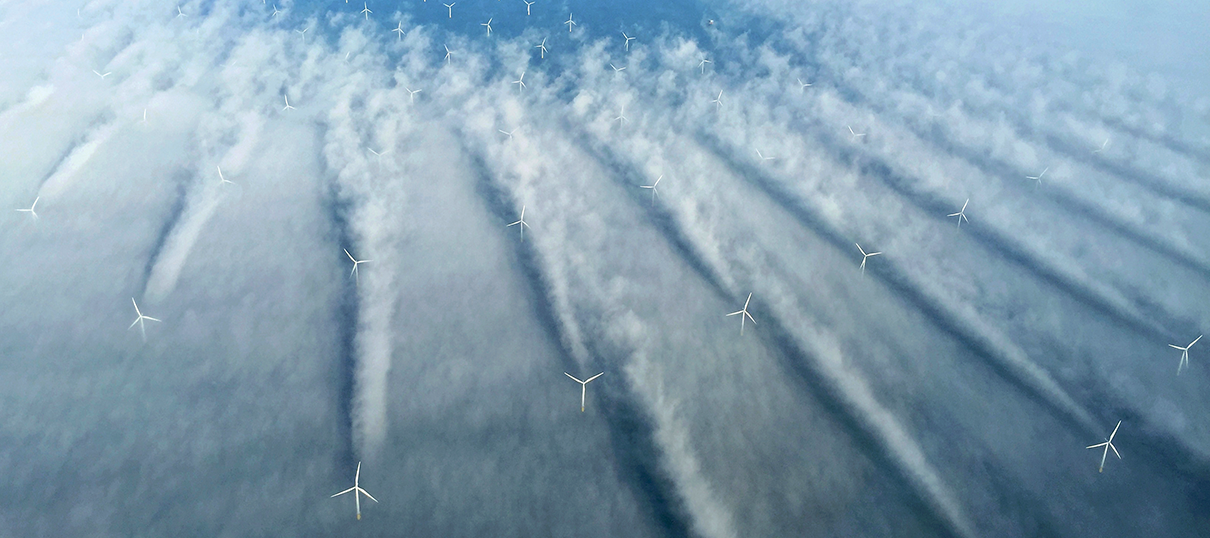
\includegraphics[width=0.8\textwidth]{figures/introduction/wake_photo.png} 
	\caption{Visible wind turbine wakes due to contrail generation \cite{windpowermonthly_offshore_clusters}}
	\label{fig:wake_photo}
\end{figure}


With the overall goal of creating a model that models how the interaction between wind turbines (induced by the wake) is related to the wind turbines relative positioning to each other and the wind conditions as input to a optimization model, a tailor made dataset from simulation results is the easiest to handle to ensure that the data fits the use case well. Using self made simulation data, allows to set the parameter space of the model as required for the different variants of the optimization problems explored in the second part of this thesis. After investigating two python based open source wind farm simulation tools FLORIS (\href{https://www.nrel.gov/wind/floris}{FLORIS official website}) and PyWake (\href{https://topfarm.pages.windenergy.dtu.dk/PyWake/}{PyWake Documentation}), FLORIS was chosen after a brief comparison between the two due to an apparent ease of use. The FLORIS is a wind farm simulation tool developed by the National Renewable Energy Laboratory (NREL) as one of multiple tools containing models of varying complexity available for different use cases. FLORIS is a control-systems oriented toolbox and therefore contains a lower complexity model yielding fast simulation results. This allows the automatic generation of large quanteties of data in a relatively short time. As the data is coming from  simulation results, the data is deterministic even though there is an underlying uncertainty attributed which can be quantified by FLORIS if required. 

For this thesis, depending on the optimization problem, FLORIS is given a grid of the following parameters:

\begin{itemize}
	\item Position of Wind Turbines
	\item Wind Direction
	\item Wind Speed
	\item Wind turbolence
\end{itemize}

 defining the parameter space limits with evenly spaced data points to then generate the corresponding simulation data, with the simulation outputs being the generated power by the individual wind turbines as well as by the farm as a whole (e.g. the sum of individual power outputs). The configuation of all of these parameters as well as the number of wind turbines can be modified at will in this set up and the result is a dataset with the rows corresponding to a specific combination of parameters and the resulting power outputs of the turbines. As reference turbine, an IEA 10-MW was used due to its repeated use as baseline turbine in other scientific works like \cite{Madsen2022} and \cite{Kainz2024IEA} , a more exact technical specification can be found in \cite{Bortolotti2019}. The configurations of the specific dataset generated for the individual optimization problem formulations are documented in the corresponding Sections of Chapter \ref{section:optimization}.


\section{Modelling} \label{sec:modelling}

To model the relationship between the attributes of a incoming airflow to a wind turbine and the output generated by the same wind turbine many surrogate models could be chosen. As the model generated in this for this thesis is created with the goal of introducing it into the pyomo extension referenced in Chapter \ref{chapter:introduction}, the model has to be compatible with said extension. That is why the model chosen is a simple neural network with limited number of hidden layers and nodes, with the size of the Neural Network being limited for said extension. 

\subsection{Introduction into Neural Networks}

In the following section, a biref introduction is given into how Neural Networks work, are trained including some regularization teqniques.

\subsubsection{Arcitecture of a Neural Network}

Fundemanetally, Neural Networks represents Graph Networks consisting out of Function blocks as the nodes, in the case of Neural Networks called perceptron (or Neurons as more general terms) and arcs which correspond to the inputs/outputs of a given perceptron. In simple words, the inputs to the Neurons are summed up and introduced as argument into a function $f()$ which yields a output $y$, representing the output of the given perceptron. These Neurons are organized in layers, which correspond to the row type structure Neural Networks are usually represented in and each perceptron of one layer is connected to every other perceptron of the following layer. The following layer in this case means in the direction of flow, in visualizations usually from left to right. The arcs thus in simple terms correspond to a single number and the Neurons to the action of summing up all inputs and then applying the unspecified function $f()$ to generate a output. This process is repeated for all Neurons in the network, with the first layer of the network taking as input the values of the values of the given data features (the input values to the model) and the last layer producing outputs corresponding to the output value(s) of the model. The number of Neurons in this first and last layer correspond to the task the Neural Network is supposed to perform. If the goal is to identify handwritten numbers 1-9 from 50x50 pixel images, the imput layer might have 50x50 Neurons for the value of each pixel, and the output layer 9 layers with the output value of each perceptron representing how much the networks thinks the given image shows the corresponding numbers 1-9. A schematic of this architecture is given in Figure \ref{fig:neural_network_architecture}.

\begin{figure}[h] 
\centering
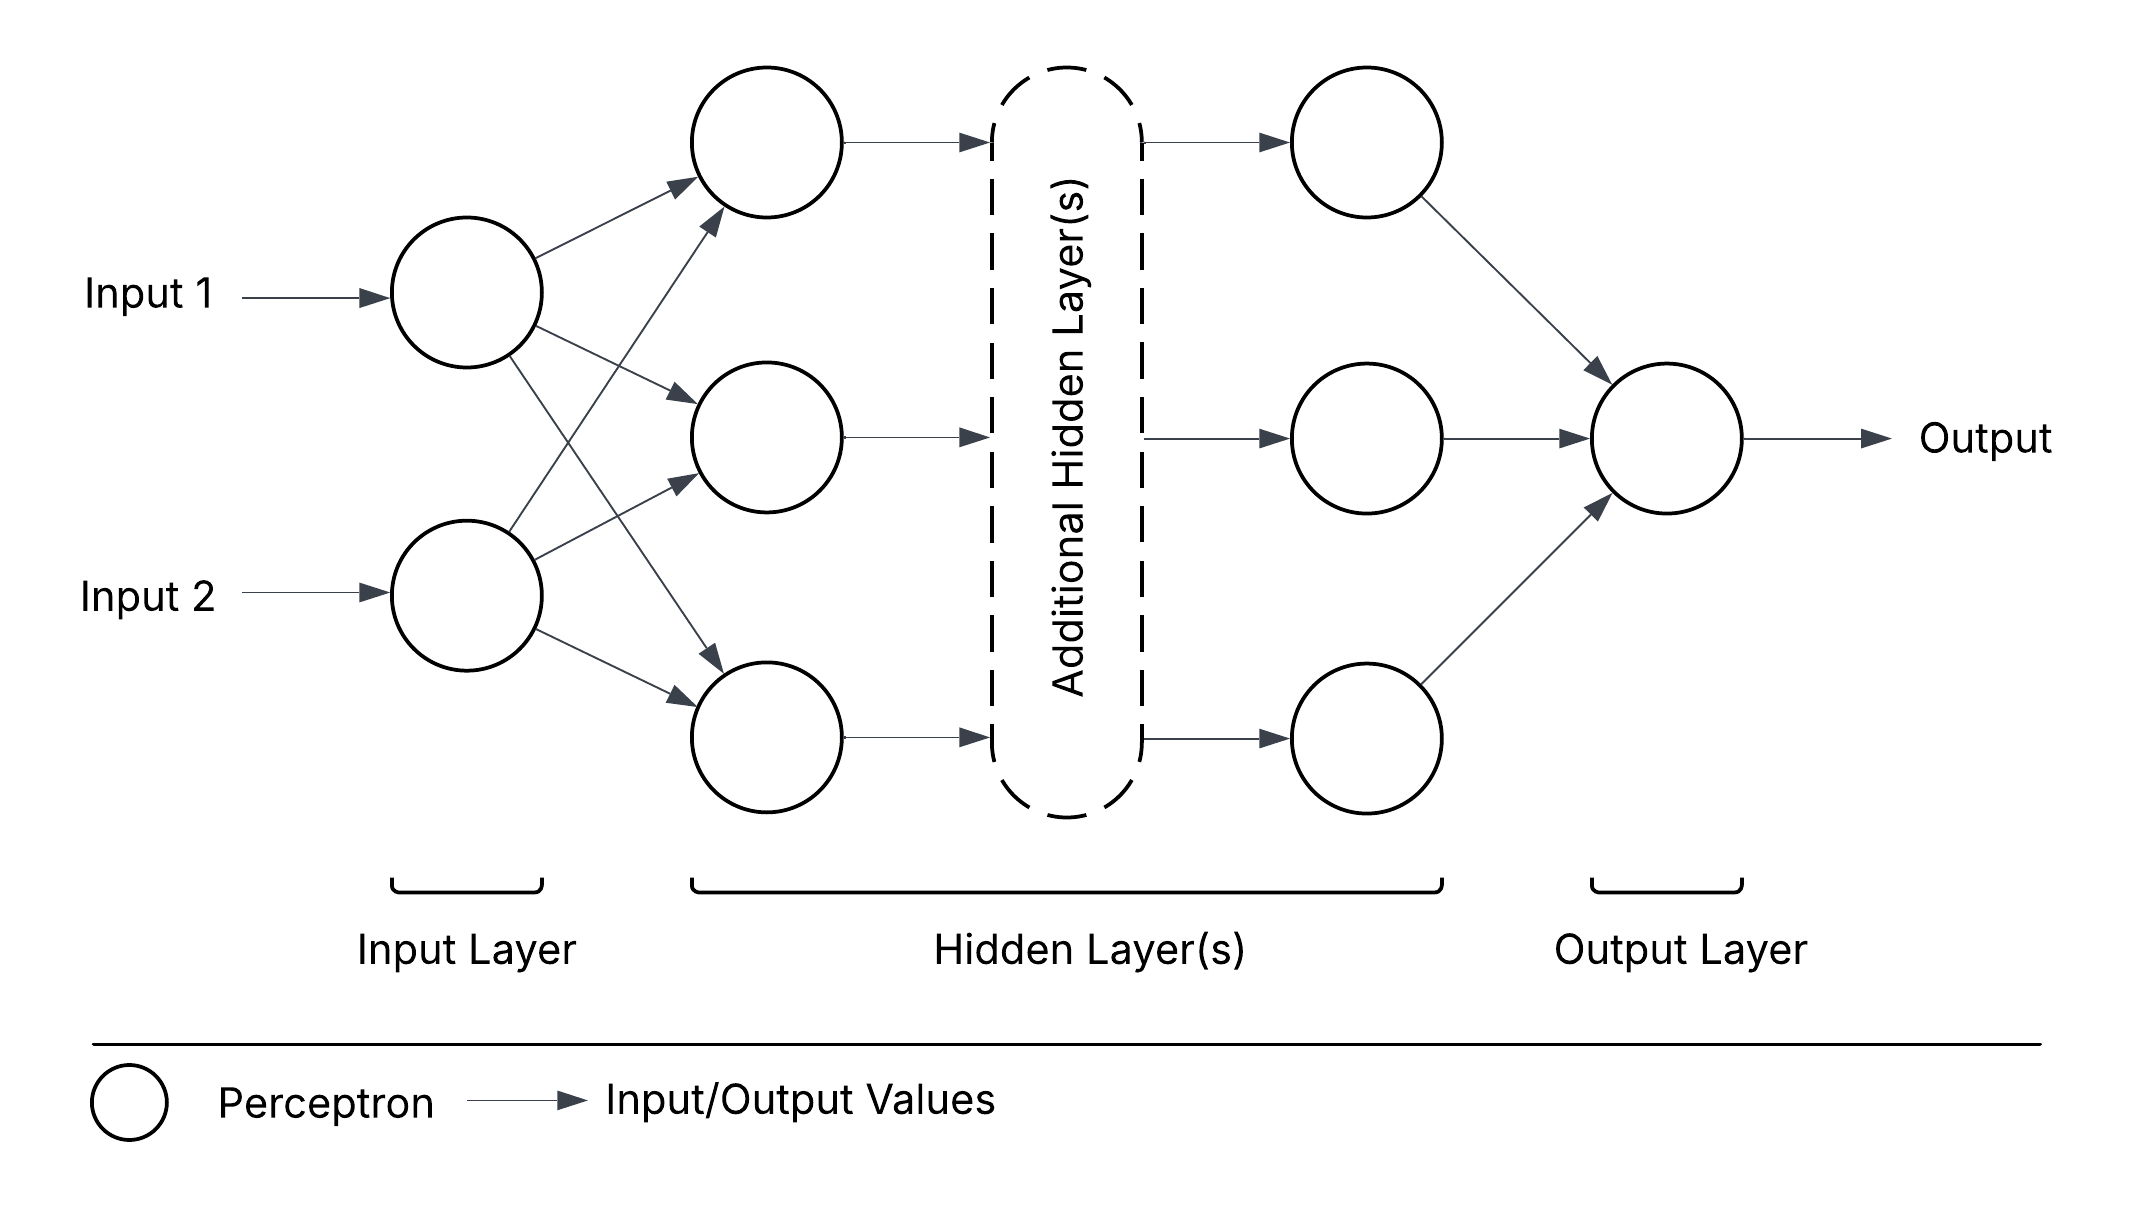
\includegraphics[width=0.9\textwidth]{figures/modelling/neural_network_concept.png} % file name without extension
\caption{Schematic of Neural Network Architecture}
\label{fig:neural_network_architecture}
\end{figure}

As shown in Figure \ref{fig:neuron_calculations} the output of a Neuron is slighlty more complicated as described befoe, as the output $y$ is generated by summing up the inputs $x$ multiplied by a corresponding weight $w$ together with a bias $b$ and introducing this summation as argument into a activation function $f()$. In this process, the weights $w$ represent a weigh to give importance to the individual inputs and the bias $b$ serves to set a minimum output value that will always be reached, regardless of the inputs. 

\begin{figure}[h] 
	\centering
	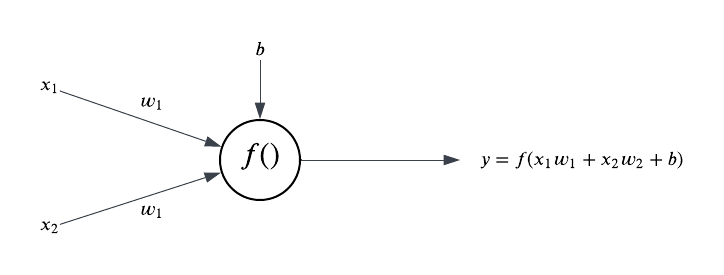
\includegraphics[width=0.8\textwidth]{figures/modelling/perceptron_concept.png} % file name without extension
	\caption{The output of a neuron is generated by applying the activation function to the sum as the weighted inputs $w_ix_i$ and the bias of the neuron $b$}
	\label{fig:neuron_calculations}
\end{figure}

The activation function $f()$ is called activation function, as in its most simplest form it represents a step function that decides if a neuron activates or not, e.g. takes the binary values ${0,1}$ for a given threshhold. Contrary to the human brain where neurons are indeed binary, most Neural Networks resort to a activation function whose outputs are not binary but deliver continious values between $0$ and $1$ to avoid the boundary issues that occour with binary threshholds. The most common function used instead of a step function is the sigmoid function, which roughly corresponds to a continuous version of the step function, with $\sigma(x) \approx 1$ for $x \to \infty$ and $\sigma(x) \approx 0$ for $x \to -\infty$.


\[
\sigma(x) = \frac{1}{1 + e^{-x}}
\]

This relationship also becomes aparent when plotting both of those functions over each other, as shown in \ref{fig:activation_functions}

\textbf{TODO: ReLU Function in text and plot}

\begin{figure}[h] 
	\centering
	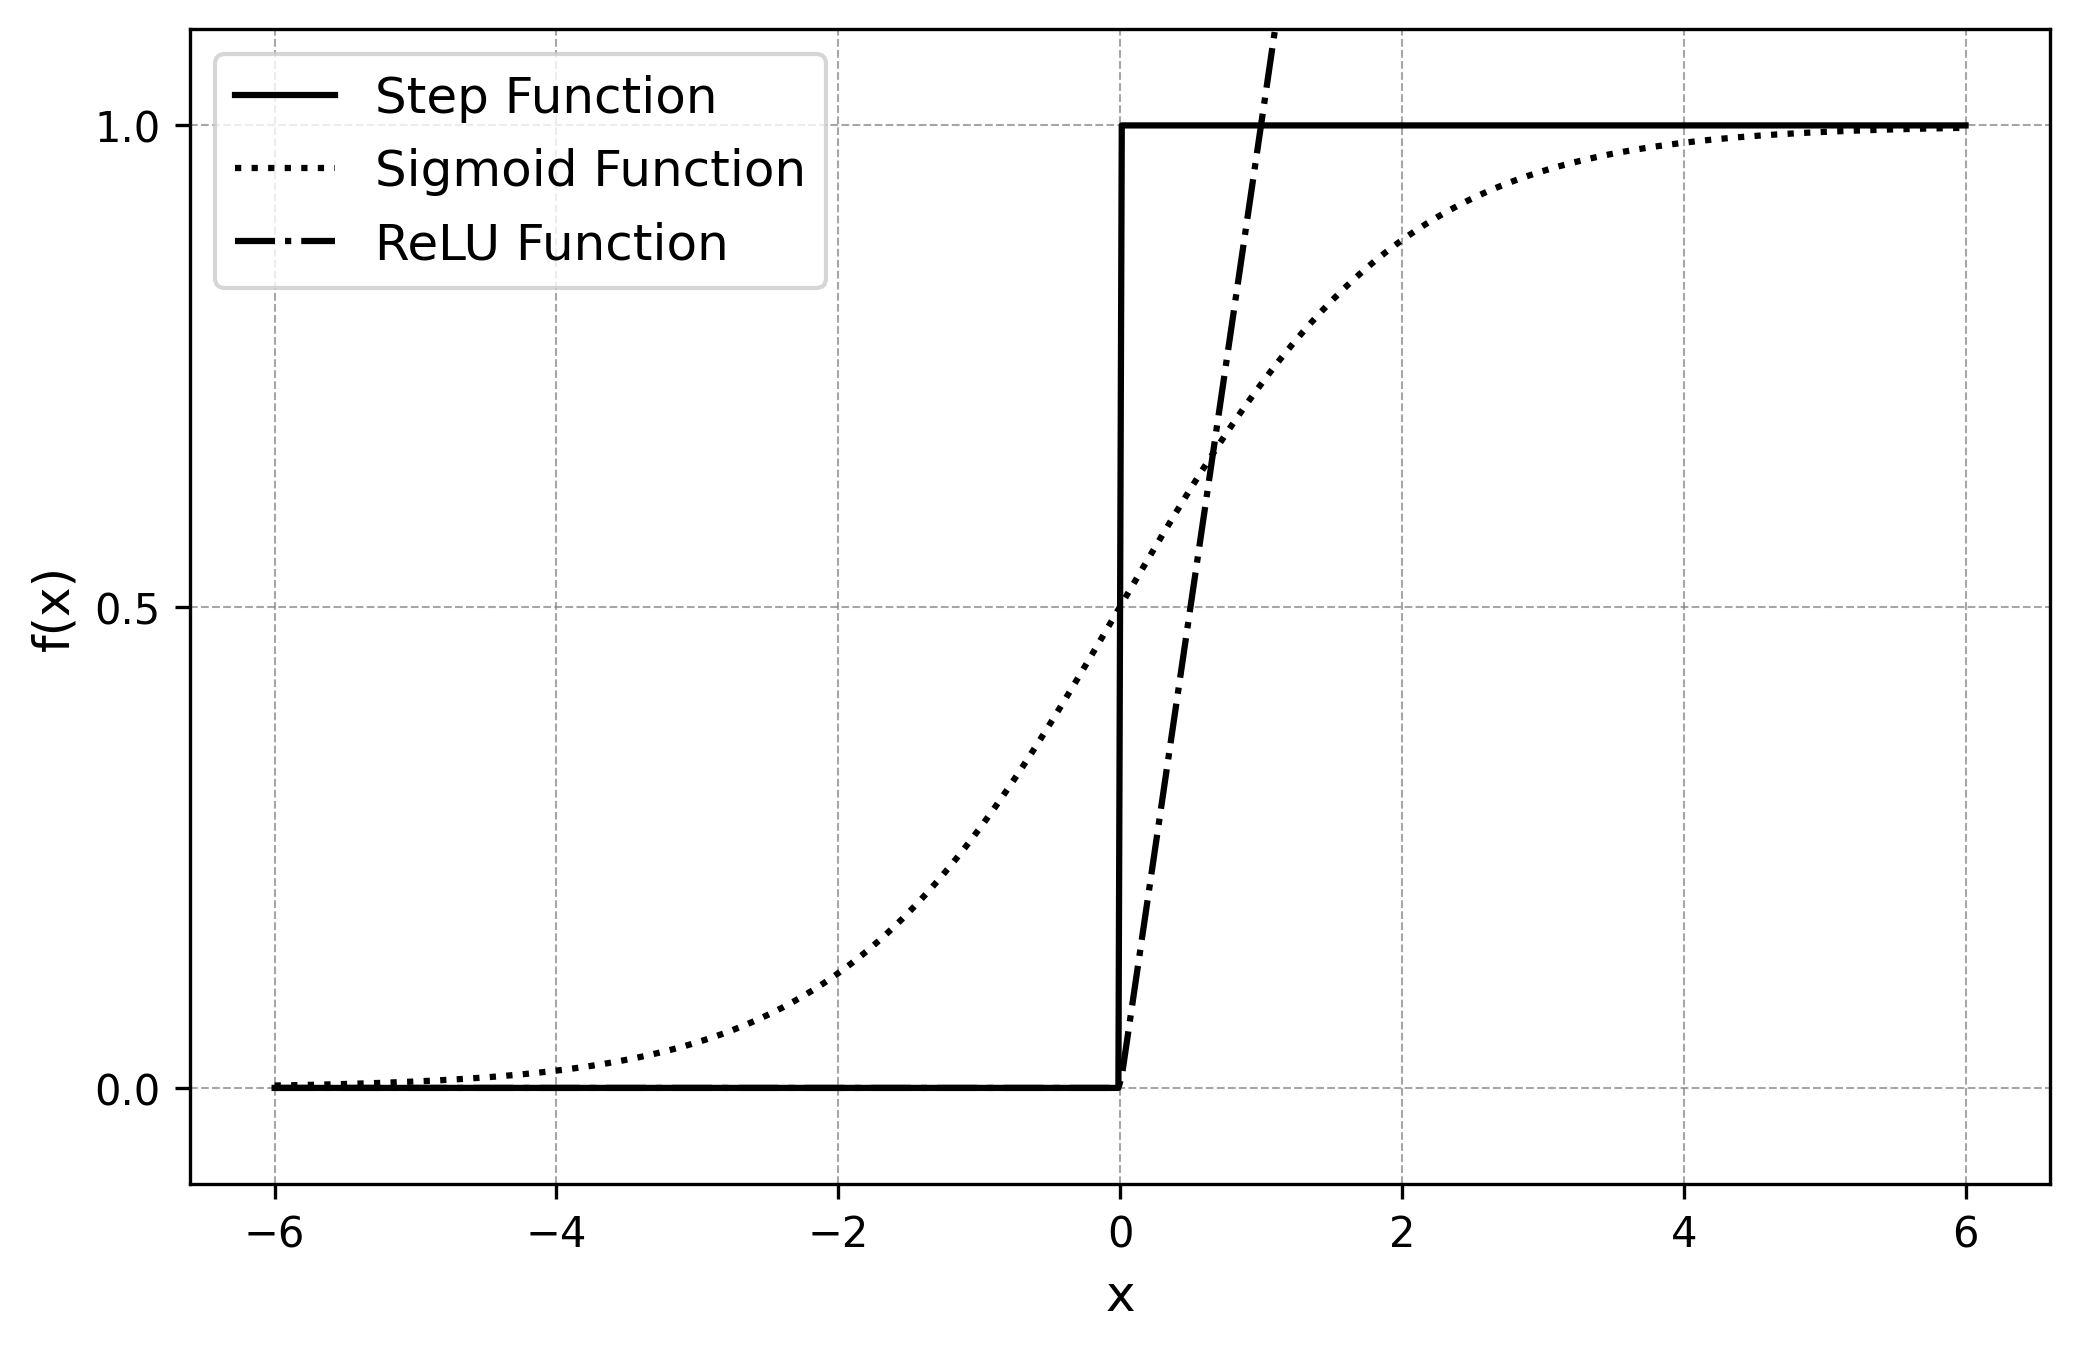
\includegraphics[width=0.9\textwidth]{figures/modelling/activation_functions.png} % file name without extension
	\caption{The Sigmoid Function being a close to the Step Function without being as sensetive to slight changes in $x$ due to its continuity}
	\label{fig:activation_functions}
\end{figure}

\cite{nielsen2015neuralChap1}


\subsubsection{Training a Neural Network}

With the general structure set up, and assuming that a layout has been chosen for the neural network (e.g. number of layers and number of their coirresponding neurons), the training of the neural network corresponds to adjusting the weights $w$ and the biases $b$ of each neuron in a way, that allows the model to perform the task it is given well. What is means for the model to perform well is defined by a \textit{Loss Function}, that defines a relationship between the output of the model and the correct output (defined by training data) and gives a Loss as output, which is some sort of delta between model prediction and truth. As what it means for a model to perform well heavily depends on the task (regression, binary classification, multiclass classification etc.), but regardless of the task, the goal is always to minimize the Loss Function. A well known Loss Function in regression is the Mean Squared Error (MSE)

\[
\text{MSE} = \frac{1}{n} \sum_{i=1}^{n} (y_i - \hat{y}_i)^2
\]

The training of the Neural Network thus corresponds to adjusting the weights and biases in a way that minimizes the chosen loss function. The algorithm most commonly used for this is called \textit{Backpropagation}.
 \cite{nielsen2015neuralChap1}
 
 Before diving into how the algorithms works exactly, it makes sense to first define specifically what parameters have to be optimized, e.g. all weights and biases of the network to be optimized. A common notation of the individual weights is as $w_{jk}^l$ with $l$ being the layer of nodes into which $w_{jk}^l$ are the weights of its inputs ( weighing the values from the outputs of the $(l-1)^{th}$ layer) and $j$ as the neuron from the $l^{th}$ layer as well as $k$ the neuron of the  $(l-1)^{th}$. Similarly, the biases are written as $b_j^l$ with $l$ as the layer and $j$ the neuron in that layer as as can be seen for both the weights and bias in an example in Figure \ref{fig:bias_and_weights_notation}.
 
 
 \begin{figure}[h] 
 	\centering
 	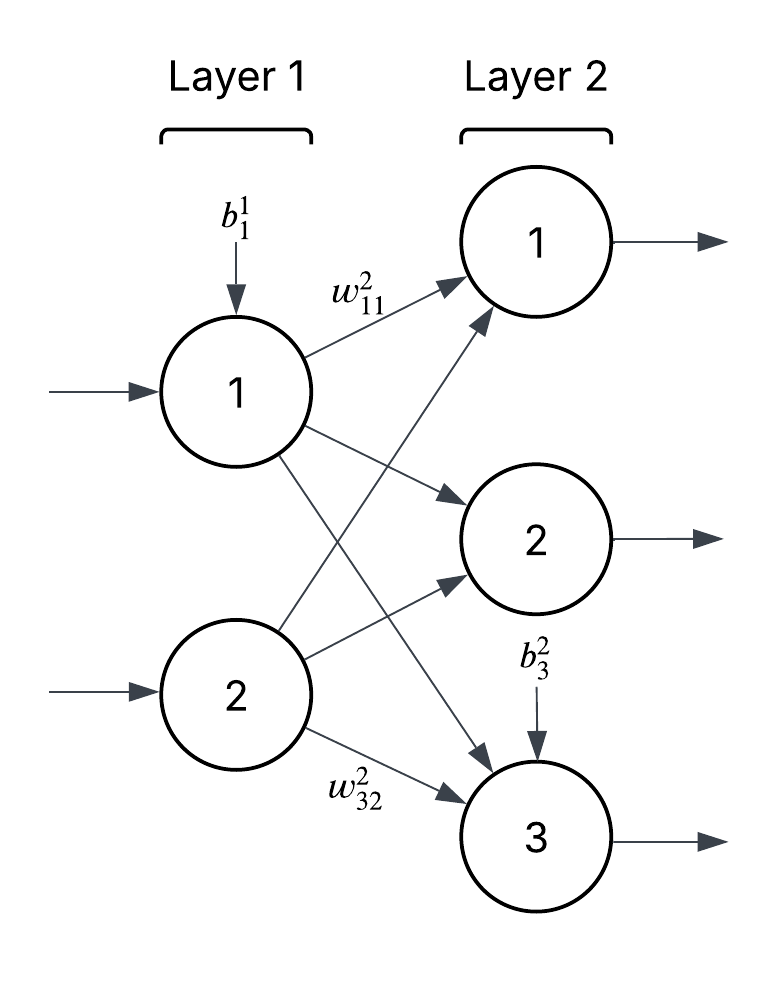
\includegraphics[width=0.4\textwidth]{figures/modelling/bias_and_weights_notation.png} 
 	\caption{Notation of Neural Network weights and biases with weight $w_{jk}^l$ and $l$ being the input layer,  $j$ the neuron from that input layer and $k$ the neuron of the  $(l-1)^{th}$ output layer. Similarly, the bias as $b_j^l$ with $l$ as the layer and $j$ the neuron.}
 	\label{fig:bias_and_weights_notation}
 \end{figure}
 (....) 
 
 Using this notation, the output of a given neuron $a_j^l$ can be calculated as 
 
 $$
 a_j^l = \sigma\left( \sum_k w_{jk}^l a_k^{l-1} + b_j^l \right),
 $$
 
 this expression can be further simplified,by writing weights and biases in matrix form, using for each layer, a weight matrix $w^l$ for all weights input into the given layer $l$ and a bias vector $b^l$. By doing so, the output vector $a^l$ of a the entire layer $l$ can be calculated as.
 
 $$a^l = \sigma (w^la^{l-1}+b^l)$$
 
With the notation for weights and biases established, the goal becomes tuning them in such a way, to minimize a chosen Loss function as discussed above. This is done by using training data with a known correct output and changing weights and Biases in such a way, that moves the Neural Network towards outputting the true known value. 
The algorithm to do so essentially corresponds to: 

\begin{enumerate}
	\item Introduce Training Data into the Neural Network
	\item Evaluate the Loss Function for the Training Points (with small random values for weights and biases for the first iteration) and evaluate the gradients of the Loss function for the gradients of the individual weights and biases ($\frac{\Delta Loss}{\Delta w_{jk}^l}$, $\frac{\Delta Loss}{\Delta b_j^l}$) using backpropagation  \footnote{The Gradient can either be evaluated for each training point individually or for batches of training points}
	\item Update the weights and biases according to a learning rate $\rho$ weighted by the specific weight or biases gradient like $w_{jk}^l =w_{jk}^l - \rho \frac{\delta Loss}{\Delta w_{jk}^l}$ and $b_j^l =b_j^l - \rho \frac{\Delta Loss}{\Delta b_j^l}$ 
	\item Repeat process $n$ Epochs, with one Epoch being the algorithm passing through all training points/batches of points once
\end{enumerate}

This algorithm represents a gradient descent algorithm with learning rate  $\rho$ corresponding to the step length, while evaluating the partial derivatives $\frac{\Delta Loss}{\Delta w_{jk}^l}$, $\frac{\Delta Loss}{\Delta b_j^l}$ is the critical step. Here the packpropagation algorithm gives an efficient method of finding these partial derivatives by evaluating the individual error contributions of each Neuron and how errors accumulate as the inputs move through the Network. A more extensive explonation of how backpropagation works can be found in \cite{nielsen2015neuralChap2}. As common for gradient descent, finding the global optimum for the weights and biases is not guaranteed and even improbable if many local minima exist as they do for the many parameters of a Neural Network. None the less, using gardient descent it can be hoped to find a good local minimum.   \cite{James2013} \cite{nielsen2015neuralChap2}

 \subsubsection{Regularization}
 
 Like for most machine learning models, Neural Networks run at risk of overfitting. Neural Networks are especially prone to overfitting due to their many degrees of freedoms represented by the many biases and weights, potentially exceeding the number of training samples.

 To prevent overfitting, regularization tecniques like Cross-Validation can be applied in training like for any other model. One very specific regularization method for Neural Networks is \textit{Dropout Learning}, which corresponds to randomly removing Neurons from the network (by effectively setting their activation function and thus their output to 0) for each training observation. By other nodes having to "stand-in" for the dropped-out nodes, nodes are prevented from developing overspecialization. \cite{James2023}



\textbf{Notes}
- many Degrees of Freedom, many local maxima
- Adaptive Moment Estimation (ADAM) optimization

\subsubsection{Neural Networks for Parametric Distributions, Quantile Neural Networks}


Distributional Neural Networks
Quantile Neural Networks

Loss for Parametric Normal: Gaussian Negative Log Likelihood


\subsection{Generating Neural Network Model for two Windturbines}

\section{Validation}
\chapter{Optimization}\label{section:optimization}

With the model of farm/turbine power established, the following section treats the embedding of the trained model(s)  into a stochastic optimization problem. The underlying theory of optimization under uncertainty and constraint learning is introduced before the actual optimization problems are defined, required models trained and results discussed.

\section{Optimization under Uncertainty}

While some things in life are certain, most are not and this is as true for optimization as for anything else. That means, that while optimizing anything from next year's crop to tomorrow's energy pricing might be done by assuming fixed values for the parameters of an optimization problem, in reality, most of these parameters contain uncertainty. The field of Stochastic Programming is occupied with finding methods that allow for introducing these uncertainties into optimization problems.

One way to approach these uncertainties is to split the problem into scenarios. A bakery for example has to decide on how many Baguettes to bake for the next day to maximize its profit. Baking too few Baguettes will lead to missing out on potential sales while baking too many baguettes will mean that the demand is fulfilled but the money invested in the excess number of baguettes is lost. Assuming the mean number of baguettes bought every day is $1000$, the price to buy a baguette is $1 €$ and the cost to produce a baguette is $0,2 €$ the classical approach to solving such a problem would be by the following formulation \footnote{$x$ of course non-negative}: 


\begin{align*}
	\max_{x} \quad \left( 1.00 \cdot \min(x,1000) - 0.20 \cdot x \right)
\end{align*}


To introduce the two scenarios additional scenarios of the demand being $10\%$ lower ($900$ Baguettes) and $10\%$ higher ($1100$ Baguettes) can be added. Assuming that the mean demand has a $50\%$ probability of occurring and the $10\%$ demand increases a $20\%$ probability and the decrease a $10\%$  probability, the problem can be modified to maximize the expected profit across these three scenarios by the formulation

\begin{align*}
	\max_{x} \quad & 0.5 \cdot \left(1.00 \cdot \min(x,1000) - 0.20 \cdot x \right) \\
	&+ 0.3 \cdot \left(1.00 \cdot \min(x,900) - 0.20 \cdot x\right) \\
	&+ 0.2 \cdot \left(1.00 \cdot \min(x,1100) - 0.20 \cdot x\right)
\end{align*}

The result from this optimization problem would be the Expected profit and how many Baguettes are the optimal number of Baguettes to yield the maximum Expected profit across all scenarios. This would be optimal assuming there exists no more information about the next day's demand, meaning that by using this approach the total profit over a long time would be maximal. In case there is more information regarding the next day's demand the probabilities that give the weights in this optimization might shift, with one scenario potentially reaching probability $100\%$ if there were to be absolute certainty that the next day's demand would be for example $1100$ baguettes. As having such exact information is however very rare, the best solution will be in most cases to maximize the profit Expectation. 

The obvious connection to conventional statistical analysis is that the demand is a random variable that can take multiple values, in this case, we assumed it to be a discrete random variable $Y$ with support ${900,1000,1100}$ even though in real-world applications the demand of baguettes will move somewhere between $[0,\infty]$. Finding the Expectation for such a discrete random variable can be done as 

\[
\mathbb{E}[X] = \sum_{i} x_i \cdot \mathbb{P}(X = x_i) = \sum_{i} x_i p_i
\]

or for continuous random variables  
 
\[
\mathbb{E}[X] = \int_{-\infty}^{\infty} x \cdot f_X(x) \, dx
\]

Using these two expressions, optimization problems can thus be formulated to optimize the Expectation of objective functions containing random variables. \cite{BirgeLouveauxStochasticProgramming}


\section{Constraint Learning} \label{sec:constraint_learning}

Constraint learning refers to introducing a model that has learned relationships between certain variables from data into an optimization problem. In the case of constraint learning, the model gets more specifically introduced into an optimization problem as part of a constraint. As many real-life relationships struggle to be represented by explicit function to be defined as objective function or constraint, introducing machine learning models to optimization problems opens up many new possibilities \cite{FAJEMISIN20241}.

In the case of Neural Networks, one way of introducing a Network as a constraint into an optimization problem is by recognizing that when using the Rectifier Linear Unit (ReLu) Function is used as an activation function with the (linear) sum of neuron bias and weighted inputs $\tilde{v}_i^\ell$ being the function argument


\begin{equation}
	v_i^\ell = \max(0, \tilde{v}_i^\ell) = \max(0,  b_i^\ell + \sum_j w_{ij}^\ell v_j^{\ell - 1})
\end{equation}


the function can be rewritten as the following constraints 

\begin{align}
	v_i^\ell &\geq \tilde{v}_i^\ell \\
	v_i^\ell &\leq \tilde{v}_i^\ell - M^{\text{low}}(1 - j_i) \\
	v_i^\ell &\leq M^{\text{up}} j_i
\end{align}

with $j_i \in \{0,1\}$ a integer variable such that

\begin{align}
	j_i =
	\begin{cases}
		0 & \text{if } \tilde{v}_i^\ell < 0 \\
		1 & \text{if } \tilde{v}_i^\ell > 0
	\end{cases}
\end{align}

This decomposition allows for introducing a Neural Network of limited size into an optimization problem by decomposing it into a set of linear constraints of the form shown above. \cite{ALCANTARA2023120895}

\section{The two Turbine Problem}

Optimizing the positioning of two wind turbines can be expressed as optimizing the relative position of a second wind turbine $T_2$ to a fixed first turbine $T_2$, defined by the relative distances $\Delta x$ and  $\Delta y$. Both  $\Delta x$ and  $\Delta y$ are constrained by minimum distance $\Delta_{min}$ to  $T_2$ and maximum distances $\Delta x_{max}$/$\Delta y_{max}$ to make the problem bounded. 
This problem can be visualized as shown in Figure \ref{fig:two_turbine_problem}.

\begin{figure}[h] 
	\centering
	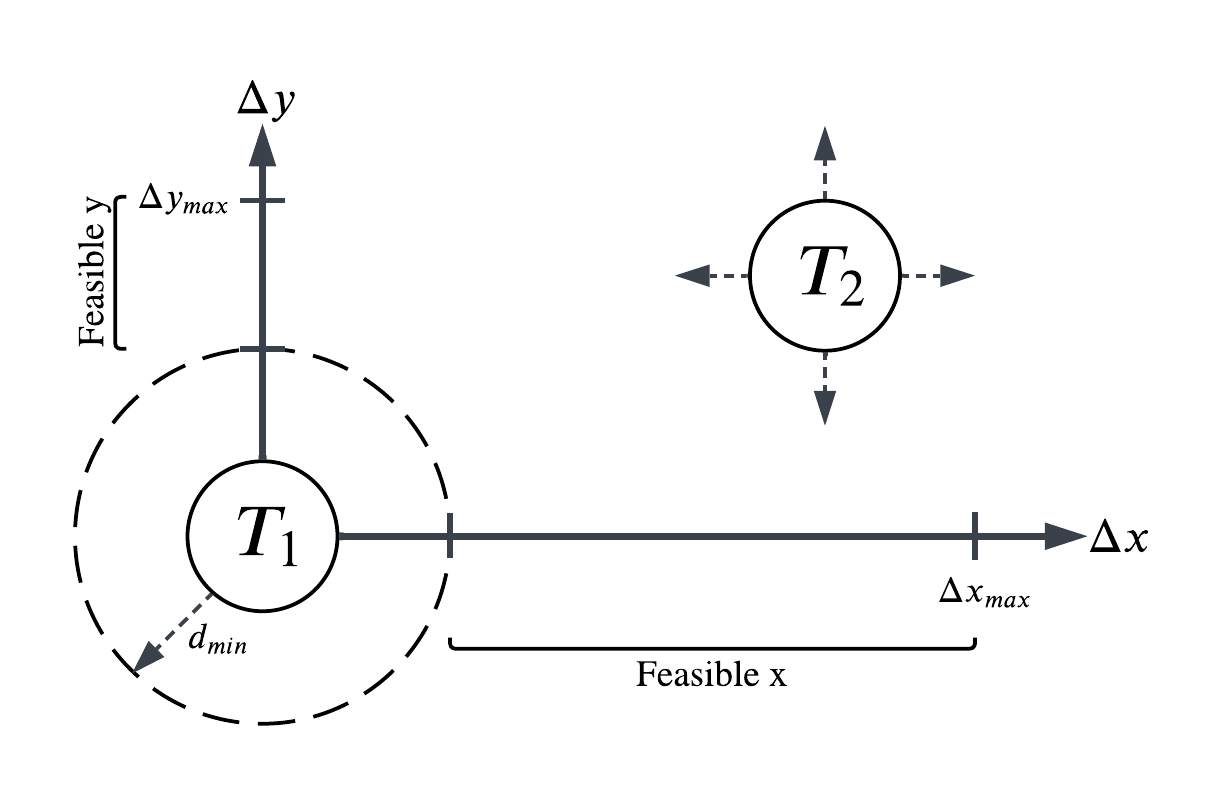
\includegraphics[width=0.6\textwidth]{figures/optimization/two_turbine_problem_schematic.png} % file name without extension
	\caption{Optimizing the relative position $\Delta x$/$\Delta y$ of a second wind turbine $T_2$ to a fixed first turbine $T_2$, constrained by minimum distance $d_{min}$ to  $T_1$ and maximum distances $\Delta x_{max}$/$\Delta y_{max}$}
	\label{fig:two_turbine_problem}
\end{figure}

The objective function to be optimized is the total power generation, e.g. the sum of power generated by both turbines. This objective is a function both of the position of the wind turbine as well as of the wind conditions like wind direction and wind speed. 

$$
f_{total Power}(x,y,\text{windspeed},\text{wind direction}, \text{(...)})
$$

Differently from the geographic coordinates, th wind condition parameters like windspeed are inherently not deterministic and follow distributions like the normal distribution as shown in Figure \ref{fig:wind_dist}.

\begin{figure}[h] 
	\centering
	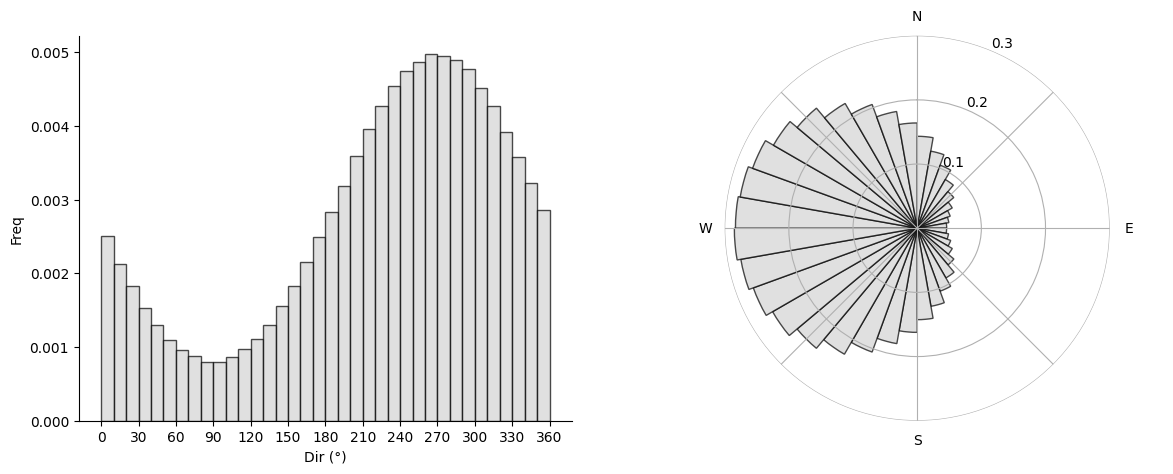
\includegraphics[width=0.9\textwidth]{figures/optimization/wind_dist.png} % file name without extension
	\caption{Histogram and Polar Plot across radiants for a normally distributed wind direction probability density function with mean West}
	\label{fig:wind_dist}
\end{figure}

The two main challenges of the optimization of the shown two turbine problem are thus: 

\begin{enumerate}
	\item Introduce the complex relationship between turbine position and wind conditions and power output into the optimization problem
	\item Introduce the non-deterministic nature of wind conditions into the optimization problem
\end{enumerate}

The first of these challenges is tackled by applying the Neural Network models discussed in Section \ref{sec:modelling} and introducing them into the optimization problem via constraint learning as described in Section \ref{sec:constraint_learning}. For the second problem, multiple approaches are now explored in the following subsection.


\subsubsection{Deterministic Optimization: Optimization for main Wind direction and Speed}

To begin solving the problem, the simplest approach is taken by assuming the wind conditions to be discrete. In application, this might be analogous to getting the Expectation of the joined probability distribution of all wind condition parameters. Taking these parameters as constant and homogeneous across the entire parameter space, the result is an objective function that is effectively only dependent on the relative positions of the turbine with the previously discussed geometrical constraints.

\begin{align}
	\max_{\mathbf{x}, \mathbf{y}} & f_{Power,\text{NN}}(\Delta x, \Delta y) \\
	\text{s.t.} \quad 
	&  \Delta x \leq X_{\max} \\
	&  \Delta y \leq Y_{\max} \\
	& \sqrt{(\Delta x)^2 + (\Delta y)^2} \geq d_{\min}
\end{align}

where:
\begin{itemize}
	\item \( (\Delta x, \Delta y) \) are the relative distances of the two turbines,
	\item \( f_{Power, \text{NN}}(\Delta x, \Delta y)\) is a neural network (deterministic) approximating the total power output ,
	\item \(  X_{\max}, Y_{\max} \) define the maximal distance the two turbines can be placed apart
	\item \( d_{\min} \) is the minimum distance between the two turbines.
\end{itemize}


When solving this problem as defined using Gurobi, a major challenge becomes apparent as the result shows that there is an infinite amount of equally optimal solutions (e.g. degeneracy of the problem, see  \cite{vanderbei2020chapter3} for an exact definition of degeneracy) everywhere outside the wake of turbine 1. This phenomenon is very intuitive when generating a heatmap of the power generation for all possible positions of turbine 2, as shown in Figure \ref{fig:two_turbine_heatmap_degeneracy}

\begin{figure}[h] 
	\centering
	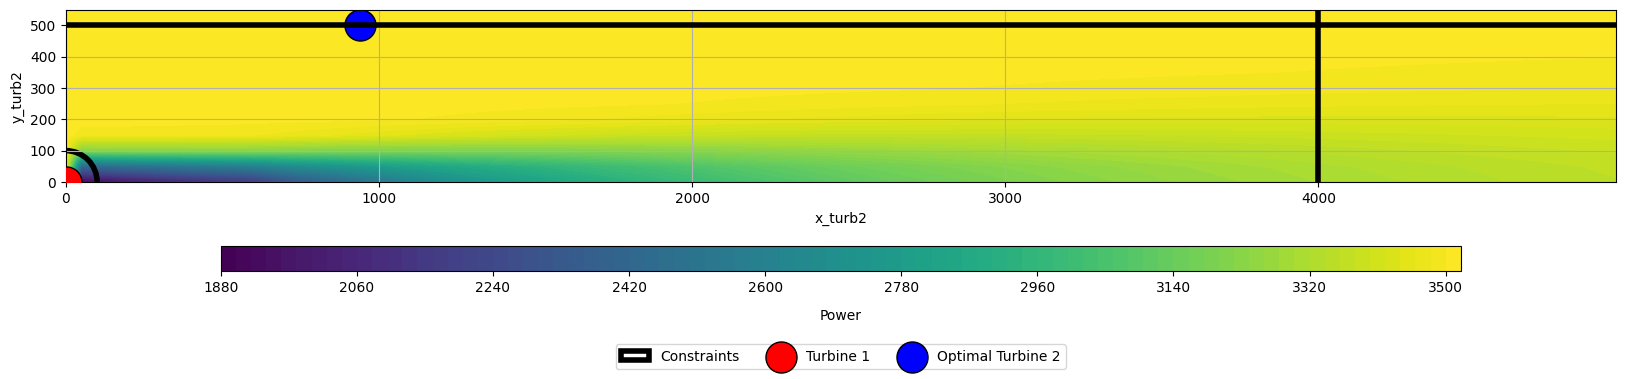
\includegraphics[width=1\textwidth]{figures/optimization/opti_determ270.png} 
	\caption{Deterministic optimization of the relative position of two windturbines relative to each other with winddirection 270° and constant windspeed}
	\label{fig:two_turbine_heatmap_degeneracy}
\end{figure}

This phenomenon will have to be kept in mind going forward while introducing a distribution for wind condition parameters might reduce the number of global optima. 


\subsubsection{Stochastic Optimization:  Power weighted by probability}

As the deterministic optimization does not take into account the distribution of wind condition parameters and having found that the deterministic approach leaves a range of infinite global optima outside of the wake of turbine 1, the next step is proceeding with the introduction of uncertainty in the form of probability distributions of wind condition parameters into the problem. This step primarily changes the objective function, which is set up such that the neural network takes in both position and wind condition parameters. the output of this neural network is then weighed by the probability of the specific wind condition occurring and the Expected power is calculated by integrating (discretized as a sum) across all combinations of wind condition parameters.

\begin{align}
	\max_{\mathbf{x}, \mathbf{y}} &  \sum_{i=1}^{n} f_{Power,\text{NN}}(\Delta x, \Delta y, \text{wind condition})\cdot p_{n,\text{wind condtion combination}} \\
	\text{s.t.} \quad 
	&  \Delta x \leq X_{\max} \\
	&  \Delta y \leq Y_{\max} \\
	& \sqrt{(\Delta x)^2 + (\Delta y)^2} \geq d_{\min}
\end{align}

where:
\begin{itemize}
	\item \( (\Delta x, \Delta y) \) are the relative distances of the two turbines,
	\item \( f_{Power, \text{NN}}(\Delta x, \Delta y)\) is a deterministic neural network  approximating the total power output for turbine positions and wind conditions
	\item \(  X_{\max}, Y_{\max} \) define the maximal distance the two turbines can be placed apart
	\item \( d_{\min} \) is the minimum distance between the two turbines
	\item \( n \) is the index of the discretized possible combinations of wind conditions 
\end{itemize}

In practice, this approach comes with challenges as it requires the constraints representing the neural network to be realized $n$ times for each wind condition combination. With one instance of the neural network already adding a significant amount of constraints to the optimization model, realizing those constraints $n$ times may lead to an overflow of constraints, making the model too difficult to solve.
	

\begin{figure}[h] 
	\centering
	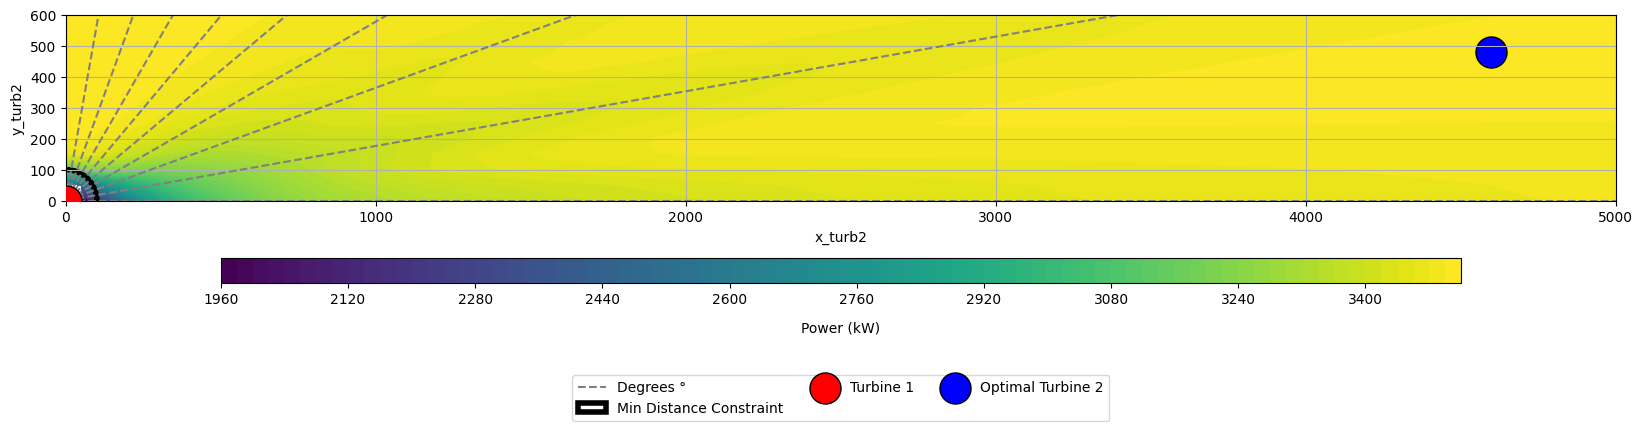
\includegraphics[width=1\textwidth]{figures/optimization/probabilistc_scenarios.png} 
	\caption{Stochastic optimization of the relative position of two windturbines relative to each other with wind normally distributed with mean $\mu = ?$ and standard deviation $\sigma = ?$, windspeed constant}
	\label{fig:two_turbine_heatmap_degeneracy}
\end{figure}
	
	
\subsubsection{Stochastic Optimization:  Power function as Quantile Neural Network}

An alternative approach to the one shown in the previous section is to implant the uncertainties of the wind condition into the power model, with the output as quantiles from a quantile neural network. 


https://pubs.aip.org/aip/aml/article/2/1/016111/3265451/Predicting-wind-farm-wake-losses-with-deep

	

\section{The three Turbine Problem}

\section{The n Turbine Problem}

Thoughts: 

IDEA: generalize inputs in a way that allow for power calculation of each turbine individually instead of farm power

IDEA : derive basic rules from 2 turbine problem and set up new optimization problem without NN 

IDEA : analogue to forward/backward selection with 2 turbine neural network


FINIDINGS: 

problem degenerate if not one wind turbine fixed

% !TeX root = ../main.tex
% Add the above to each chapter to make compiling the PDF easier in some editors.

\chapter{Conclusion}\label{chapter:conclusion}

 Once a proof of concept for the approach taken in this thesis has ben successfully performed, the data source may be eventually switched for experimental or real world data.

%\appendix{}

% % TODO: appendix chapter
%\chapter{Addenda}\label{appendix}


\chapter*{Abbreviations}
\addcontentsline{toc}{chapter}{Abbreviations}
\vspace{-0.5em} % Optional: tighten vertical space if needed


\renewcommand{\arraystretch}{1.5}
\noindent
\begin{tabular}{@{}ll@{}}
	\textbf{Abbreviation} & \textbf{Meaning} \\
	\hline
	AEP & Annual Energy Production \\
	MSE & Mean Squared Error \\
	ReLu & Rectified Linear Unit \\
	IEA & International Energy Agency \\
	MW  & Mega Watt \\
\end{tabular}
\vspace{-1em} % Optional: to avoid pushing to next page
\clearpage % Ensures the next chapter starts on a new page


\microtypesetup{protrusion=false}
\listoffigures{}
%\listoftables{}

% Bibliography
\bibliographystyle{plain}  % Use a BibTeX style (e.g., plain, alpha, apa, etc.)
\bibliography{bibliography}


\end{document}
